\chapter{VM-centric Storage Management with Approximate Deletion}
\label{chap:data}
\section{Introduction}
\label{data:intro}
In this chapter, we discuss a low-cost storage and management architecture that collocates
a backup service with other cloud services and uses a minimum amount of resources. 
We also consider the fact that after
deduplication, most data chunks are shared by several to many virtual machines.
Failure of a few shared data chunks can have a 
broad effect and many
snapshots of virtual machines could be affected.
The previous work in deduplication focuses on the efficiency and approximation of
fingerprint comparison, and has not addressed fault tolerance issues  together with deduplication.
Thus we also seek deduplication options that yield better fault isolation.
Another issue considered is that
that garbage collection after deletion of old snapshots also competes for computing resources. 
Sharing of data chunks among by multiple VMs needs to be detected during
garbage collection and such dependencies complicate deletion operations. 

The key contribution of this work is the development and analysis of a VM-centric approach
which considers fault isolation and integrates multiple duplicate detection strategies
supported by similarity guided local deduplication
and popularity guided global deduplication. 
This approach localizes duplicate detection within each VM  
and packages only data chunks from the same VM into a file system block as much as possible.
By narrowing duplicate sharing within a small percent of common data chunks and exploiting their popularity,
this scheme can afford to allocate extra replicas of these shared chunks for better
fault resilience while sustaining competitive deduplication efficiency.
In addition, our VM-centric design allows garbage collection to be performed in a localized
scope and we propose an approximate deletion scheme to reduce this cost further.
Localization also brings the benefits of greater ability to exploit parallelism so
backup operations can run simultaneously without a central  bottleneck.
This VM-centric solution uses a small amount of  memory while delivering reasonable deduplication efficiency. 

The rest of this chapter is organized as follows.
Section~\ref{data:options} reviews the background and discusses the design options for snapshot backup 
with a VM-centric approach. 
Section~\ref{data:arch} describes our system architecture and implementation details.
Section~\ref{data:analysis} analyzes the tradeoff and benefits of our approach. 
Section~\ref{data:deletion} describes out approximate deletion algorithm.
%   the benefit of our approach for fault isolation. 
Section~\ref{data:impl} is our experimental evaluation that compares with other approaches.
Section~\ref{data:related} reviews the related works.
Section~\ref{data:concl} concludes this chapter.

\section{Design Considerations}
\label{data:options}
Our key design consideration is VM dependence minimization during deduplication 
and file system block management.
\begin{itemize}
\item {\em Deduplication localization.}
Because a data chunk is compared with fingerprints collected from all VMs during
the deduplication process, only one copy of duplicates is stored in the storage,
this artificially creates data dependencies among different VM users. 
Content sharing via deduplication affects fault isolation since machine failures happen periodically 
in a large-scale cloud and
loss of a small number of shared data chunks can 
cause the unavailability of snapshots for a large number of virtual machines.
Localizing the impact of deduplication can increase fault isolation and resilience.
Thus from the fault tolerance point of view,  duplicate sharing among multiple VMs is 
discouraged. 
Another disadvantage of sharing is that it complicates snapshot deletion, 
which  occurs frequently when snapshots expire regularly. 
The mark-and-sweep approach~\cite{Guo2011,Fabiano2013}  is effective for deletion, but still carries a significant cost
to count if a data chunk is still shared by other snapshots. 
Localizing deduplication can  minimize data sharing and simplify deletion while sacrificing 
deduplication efficiency, and  can facilitate parallel execution of snapshot operations.
\item{\em  Management of file system blocks.}
The file system block (FSB) size in a distributed file system such as  Hadoop and GFS is uniform and large (e.g.  64MB),
while the data chunk in a typical deduplication system is of a non-uniform size with 4KB or 8KB on average.
Packaging data chunks to an FSB can create more data dependencies among VMs
since a file system block can be shared by even more VMs.
Thus we need to consider a minimum association of FSBs to VMs in the packaging process.
\end{itemize}

Another consideration is the computing cost of deduplication.
Because of collocation of this snapshot service with other existing cloud services, 
cloud providers will want the backup service to only consume small resources
with a minimal impact to the existing cloud services.
The key resource for signature comparison  is memory for storing the fingerprints. 
We will consider the approximation techniques with reduced memory consumption along 
with the fault isolation considerations discussed below. 

We call the traditional deduplication approach as VM-oblivious (VO)
because they compare fingerprints of snapshots without consideration of VMs.
With the above  considerations in mind, we study a 
VM-centric approach (called VC)
for a collocated backup service with resource usage friendly
to the existing applications.  

We will first present an VM-centric architecture and implementation design with deletion support 
that can be integrated with our multi-level selective deduplication scheme, then
discuss and analyze the integration of the VM-centric deduplication strategies with fault isolation.

\section{Snapshot Storage Architecture}
\label{data:arch}
\subsection{Components of a Cluster Node}
\label{data:node}
Our VM cloud runs on a cluster of Linux machines with Xen-based VMs and
an open-source package for the distributed file system  called QFS~\cite{michael2013}. 
All data needed for the backup service including snapshot data and metadata
resides in this distributed file system. 
One physical node hosts tens of VMs, each of which accesses its virtual machine disk image through the
virtual block device driver (called TapDisk\cite{Warfield2005} in Xen).

As depicted in Figure~\ref{fig:arch_vm}, 
there are four key service components running on each cluster
node  for supporting backup and deduplication: 
1) a virtual block device driver, 2) a snapshot deduplication agent,
3) a snapshot store client to store  and access snapshot data,
and 4)  a PDS client to support PDS metadata access. 

We use the virtual device driver in Xen that employs a bitmap to track the changes 
that have been made to the virtual disk (CBT).
Every bit in the bitmap represents a fixed-sized (2MB) segment, indicating whether the segment
has been modified since last backup. 
Segments are further divided into variable-sized chunks (average 4KB) 
using a content-based chunking algorithm~\cite{frame05}, 
which brings the opportunity of fine-grained deduplication.
When the VM issues a disk write, the dirty bit for the corresponding segment is set
and this indicates such a segments needs to be checked during snapshot backup. 
After the snapshot backup is finished, the driver resets the dirty bit map to a clean state.
For data modification during backup, copy-on-write protection is set so that backup can continue to
copy  a specific version while new changes are recorded.
%copies a frozen version while the modification can still carry on.

The representation of each snapshot has  a two-level index data structure.
The snapshot meta data (called snapshot recipe) contains a list of segments, each of which contains segment
metadata of its chunks (called segment recipe).
In snapshot and segment recipes, 
the data structures  include references to the actual data location to eliminate the need for additional indirection.

\begin{figure}[htbp]
    \centering
    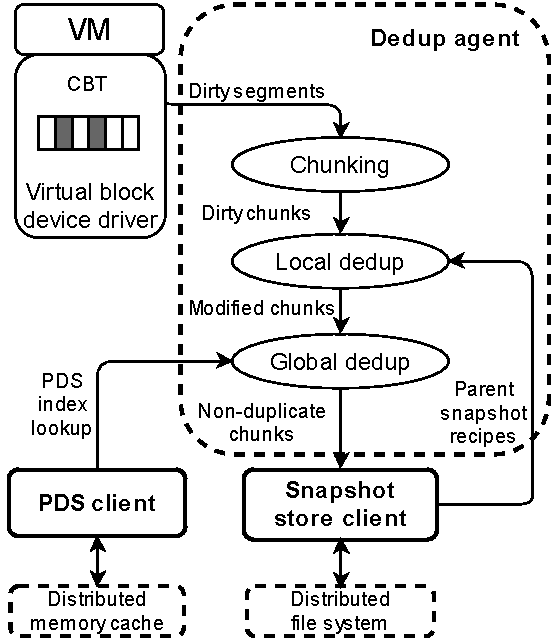
\includegraphics[width=4in]{images/socc_arch_cluster}
    \caption{System architecture and data flow during snapshot backup}
    \label{fig:arch_vm}
\end{figure}

\subsection{A VM-centric Snapshot Store for Backup Data}
\label{data:store}
We build the snapshot storage on the top of a distributed file system.
Following the VM-centric idea for the purpose of fault isolation,
each VM has its own snapshot store, containing new data chunks which are considered
to be non-duplicates.
As shown in Figure~\ref{fig:as_arch}, we explain the data structure of the snapshot stores as follows.
\begin{figure}[htbp]
  \centering
  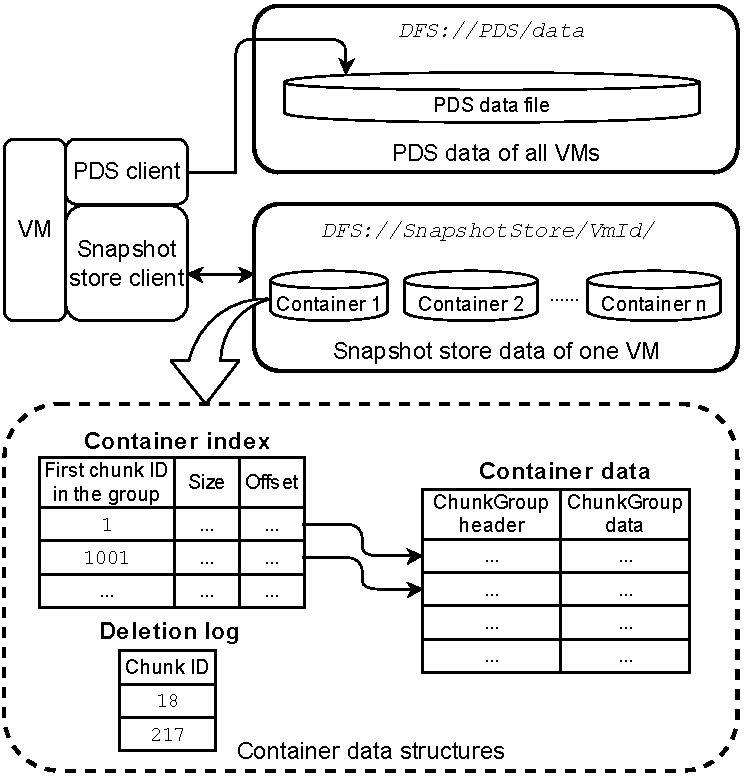
\includegraphics[width=4in]{images/sstore_arch}
  \caption{Data structure of a VM snapshot store.}
  \label{fig:as_arch}
\end{figure}

%\begin{itemize}
%\item
There is an independent store containing all PDS chunks shared among different VMs as
a single file.
%All PDS chunks are stored in one PDS file. 
Each reference to a PDS data chunk in the PDS index is the offset within the PDS file.
%There is an option to use a data structure similar to the non-PDS store. We opt
%for the simpler format because
Additional compression is not applied because 
for the data sets we have tested, we only observed limited spatial locality 
among popular data chunks. On average the number of consecutive PDS index hits is lower than 7.
Thus it is not very effective to group a large number of chunks as a compression and data fetch unit. 
For the same reason, we decide not to take the sampled index approach~\cite{Guo2011} 
for detecting duplicates from PDS as limited spatial locality is not sufficient to enable
effective prefetching for sampled indexing.

PDS data are re-calculated periodically, but 
the total data size is small.  When
a new PDS data  set is computed, the in-memory PDS index is replaced, but 
the PDS file on the disk appends the  new PDS data identified and the growth of this file is very slow. 
The old data are not removed because they can still be referenced by the existing snapshots. 
A periodic cleanup is conducted  to remove unused PDS chunks (e.g. every few months). 

%\end{itemize}

For non PDS data, the snapshot store of a VM is  divided into a set of containers and 
each container is approximately 1GB. 
The reason for dividing the snapshot store into containers is to simplify the compaction process
conducted periodically. As discussed later, data chunks are deleted from old snapshots
and chunks without any reference from other snapshots can be removed by this compaction process.
By limiting the size of a container, we can effectively control the length of each round of compaction.
The compaction  routine can work on one container at a time and move the in-use data chunks to another container. 

Each non-PDS data container is further divided into a set of chunk data groups. Each chunk group is composed of
a set of data chunks and is the basic unit in data access and retrieval. 
In writing a chunk during backup, the system accumulates data chunks and stores the entire
group as a unit after compression. This  compression can reduce data by several times  in our tested data.
When accessing a particular chunk, its chunk group is retrieved from the storage
and decompressed. Given the high spatial locality and usefulness of prefetching  in 
snapshot chunk accessing~\cite{Guo2011,foundation08},
retrieval of  a data chunk  group naturally works well with prefetching. 
A  typical chunk group contains 1000 chunks in our experiment.
% with an average size of 200-600 chunks.

%\item
Each non-PDS data container is represented by three files in the DFS:
1) the container data file holds the actual content, 
2) the container index file is responsible for translating a data reference
into its location within a container, and 
3) a chunk deletion log file records all the deletion requests within  the container.

%\item
A non-PDS data chunk reference stored in the index of snapshot recipes
is composed of two parts: a container ID with 2 bytes and a local chunk ID with 6 bytes.
Each container maintains a local  chunk counter and assigns the current number 
as a chunk ID  when  a new chunk is added to this  container. 
Since data chunks are always appended to a snapshot store during backup, 
local chunk IDs are monotonically increasing.
When a chunk is to be accessed, the segment recipe contains a reference pointing to  a data chunk
in the PDS store or in a non-PDS VM snapshot  store. 
Using  a container ID, the corresponding container index file of this VM is accessed and 
the chunk group is identified using a simple chunk ID range search. Once the chunk group is loaded to memory, 
its header contains the exact offset of the corresponding chunk ID and the content is then accessed from the memory buffer.

Our snapshot store supports three API calls for block data operations:
%\begin{itemize}

%\item
\noindent\textbf{Append()}. 
For PDS data, the chunk is appended to the end of the PDS file and the offset is returned as the  reference.
Note that PDS append may only be used during PDS recalculation.
For non-PDS data, this call places a chunk into 
the snapshot store and returns a reference to be stored in 
the recipe metadata of a snapshot. 
The write requests to append data chunks to a VM store are accumulated at the client side. 
When the number of write requests reaches a fixed group size, the snapshot store client compresses
the accumulated   chunk group, adds a chunk group index  to the beginning of the group, and then
appends the header and data  to the corresponding VM file.
A new container  index entry is also created for each chunk group and is written to the corresponding
container index file.

%\item
\noindent\textbf{Get()}.
The fetch operation for the PDS data chunk is straightforward since each reference contains 
the file offset, and the size of a PDS chunk is available from a segment recipe.
We also maintain a small data cache for the PDS data service to speedup common data fetching.
To read a non-PDS chunk using its reference with container ID and local chunk ID,  the snapshot store client first loads the
corresponding VM's container index file specified by the container ID, then searches the chunk
groups  using their  chunk ID coverage.
After that, it reads the identified chunk group from DFS, decompresses it, and seeks to the exact chunk data 
specified by the chunk ID. 
Finally, the client updates its internal chunk data cache with the newly loaded content to 
anticipate future sequential reads.

%\item
\noindent\textbf{Delete()}.
Chunk deletion occurs when a snapshot expires or gets deleted explicitly by a user and we discuss this in more details in next
subsection.
%(we will discuss the snapshot deletion in detail in the following subsection).
When deletion requests are issued for a specific container,
those requests are simply recorded into the  container's deletion log initially and thus  a lazy
deletion strategy is exercised.
Once local chunk IDs appear in
the deletion log, they will not be referenced by any future snapshot and can be safely deleted when needed. 
This is ensured because we only dedup against the direct parent of a snapshot, so the deleted snapshot's blocks
will only be used if they also exist in other snapshots.
Periodically, the snapshot  store identifies those containers with an excessive
number of deletion requests to  compact and  reclaim the corresponding disk space. 
During compaction, the snapshot store creates a new container (with the same container ID) to replace the 
existing one. This is done by sequentially scanning the old container, copying all the chunks that are not 
found in the deletion log to the new container, and creating new chunk groups and indices. 
Every local chunk ID however is directly copied rather than re-generated. This
process leaves holes in the chunk ID values, but preserves the order and IDs of chunks.
As a result, all data references stored 
in recipes are permanent and stable, and the data reading process
is as efficient as before. Maintaining the stability of chunk IDs also ensures that recipes do not
depend directly on physical storage locations, which simplifies data migration.
%\end{itemize}

Additional APIs such as \textbf{Scan()}, \textbf{Compact()}, \textbf{Create()} and \textit{Remove()} are provided for 
higher level operations. Scan() is used by the map-reduce procedure to collect the most popular blocks among all snapshot stores.
Compact() is called when the system determines a container has too much unclaimed space and needs to be reclaimed.
Create() and Remove() initialize and delete a container respectively.

\section{Analysis of VM-centric Approach}
\label{data:analysis}
In this section we give out analysis of the impacts of our VM-centric deduplication scheme. 
As introduced in chapter~\ref{inline:dedup}, our VM-centric approach put the cluster wide 
popular data into PDS which prevent each VM from keeping their own copies. We will show that by adding
extra replication to PDS data, this strategy brings advantages to both fault tolerancy and deduplication efficiency.
The parameters we will use in our analysis below are defined in Table~\ref{tab:symbol}. 

\begin{table}[htbp]
\centering
\tabcolsep=0.11cm
\begin{tabular}{|p{1.5cm}|p{11cm}|}
\hline
$k$ &  the number of top most popular chunks selected for deduplication\\ 
\hline
$c$ &  the total amount of data chunks in a cluster of VMs\\ 
\hline
$c_u$ &  the total amount of unique fingerprints after perfect  deduplication\\
\hline
$f_i$ &  the frequency for the $i$th most popular fingerprint\\
\hline
$\delta$ &  the percentage of duplicates detected in local deduplication\\
\hline
$\sigma$ & =$\frac{k}{c_u}$ which is  the percentage of unique data  belonging to  PDS\\
\hline
$p$ & the number of machines in the cluster\\
\hline
$V$ & the average number of VMs per machine\\
\hline
$E_c, E_o$ & deduplication efficiency of VC and VO \\
%\hline
%$D$ & the amount of unique data on each machine\\
%\hline
%$s$ & the average data chunk size. Our setting is  4K.\\
\hline
$s$ & the average number of chunks per FSB\\
%\hline
%$m$ & memory size on each node used by VC\\ 
%\hline
%$E$ & the size of an popular data index entry\\
\hline
$N_1$ & the average number  of non-PDS FSBs blocks in a VM for VC\\
\hline
$N_2$ & the average number  of PDS FSBs in a VM for VC\\
\hline
$N_o$ & the average number  of FSBs  in a VM for VO\\
\hline
A(r) & the availability of an FSB  with replication degree $r$\\
\hline
\end{tabular}
\caption{Modeling  parameters}
\label{tab:symbol}
\end{table}

\subsection{Impact on Deduplication Efficiency}
Choosing the value $k$ for the most popular chunks affects the deduplication efficiency.
We analyze this impact based on the characteristics  of the VM snapshot traces
studied from  application datasets.
A previous study shows that the popularity of data chunks after local deduplication follows 
a Zipf-like distribution\cite{Breslau1999a, Baek2011} and its
exponent $\alpha$ is ranged between 0.65  and  0.7~\cite{WeiZhangIEEE}. 
Figure~\ref{fig:zipf-data} illustrates the Zipf-like distribution of chunk popularity.

%Table~\ref{tab:symbol} defines paramters $c$, $c_u$, $f_i$, and $\delta$ used below.
%let $c$ be the total number of data chunks. 
%$c_u$ be the total number of fingerprints 
%in the global index after complete deduplication, and
%$f_i$ be the frequency for the $i$th most popular fingerprint. 
By Zipf-like distribution, $f_i = {f_1}/{i^\alpha}.$
The total number of chunks in our backup storage which
has local duplicates excluded is $c (1-\delta)$, this can be represented
as the sum of each unique fingerprint times its frequency:
%Since $ \sum_{i=1}^{c_u}f_i = c (1-\delta)$,
\[
f_1 \sum_{i=1}^{c_u}\frac{1}{i^\alpha} = c (1-\delta).
\]
Given $\alpha <1$, $f_1$ can be approximated with integration:
%\begin{equation}
\[
f_1=\frac{c(1-\alpha)(1-\delta)}{c_u^{1-\alpha}}.
\]
%\end{equation}

Thus putting the $k$ most popular fingerprints into PDS index can remove the following number of chunks during global 
deduplication:
\[
f_1 \sum_{i=1}^{k}\frac{1}{i^\alpha} \approx  
f_1 \int_{1}^{k}\frac{1}{x^\alpha} dx  \approx  f_1\frac{  k^{1-\alpha}} {1-\alpha}
=c(1-\delta) \sigma^{1-\alpha}.
\]

Deduplication efficiency of the VC approach using top $k$ popular chunks
is the percentage of duplicates that can be detected:  
\begin{equation}
\label{eq:dedupeff}
%\begin{split}
%e_k &= 
E_c=\frac{ c\delta + c(1-\delta) \sigma^{1-\alpha}}
{c  - c_u }.\\
%\end{split}
\end{equation}

% After the global deduplication, the number of remaining chunks is:
% \[
% c-E(c-c_u)
% \] 

We store the PDS index using a distributed shared memory hash table such as Memcached
and allocate a fixed percentage of memory space per physical machine for top $k$ popular items.
As the number of physical machines ($p$) increases,
the entire cloud cluster can host more VMs; however,  ratio $\sigma$ which is $k/c_u$ remains
a constant because each physical machine on average still hosts a fixed constant number of 
VMs. Then the overall deduplication efficiency of VC defined in Formula~\ref{eq:dedupeff}
remains constant.
Thus the deduplication efficiency is stable  as $p$ increases as long as $\sigma$  is a constant.


\begin{figure}[htbp]
  \centering
    \begin{tikzpicture}
            \begin{axis}[
            %title={PDS Coverage},
            width=0.7\linewidth,
            height=0.5\linewidth,
            cycle multi list={
                mline\nextlist
                [3 of]mmark*\nextlist
            },
            %cycle list name=mcolor,
            xlabel={Total num. chunks stored (in billions)},
            ylabel={PDS Coverage (\%)},
            %extra y ticks={4.5,5.5,6.5} %to add extra ticks
            mark options=solid,
            %legend pos=outer north east,
            legend columns=2,
            legend style={
                at={(0.5,-0.30)},
            anchor=north},
            ]
            \addplot table[x expr=\thisrow{InputChunks}/1000000000,y=A1] {data/cds_coverage.txt};
            \addplot table[x expr=\thisrow{InputChunks}/1000000000,y=A2] {data/cds_coverage.txt};
            \addplot table[x expr=\thisrow{InputChunks}/1000000000,y=A4] {data/cds_coverage.txt};
            \addplot table[x expr=\thisrow{InputChunks}/1000000000,y=T1] {data/cds_coverage.txt};
            \addplot table[x expr=\thisrow{InputChunks}/1000000000,y=T2] {data/cds_coverage.txt};
            \addplot table[x expr=\thisrow{InputChunks}/1000000000,y=T4] {data/cds_coverage.txt};
            \legend{Measured ($\sigma=1\%$),Measured ($\sigma=2\%$),Measured ($\sigma=4\%$),Predicted ($\sigma=1\%$),Predicted ($\sigma=2\%$),Predicted ($\sigma=4\%$)};
            \end{axis}
    \end{tikzpicture}
  \caption{Predicted vs. actual PDS coverage as data size increases.}
  \label{fig:cds-coverage}
\end{figure}
Ratio $\sigma^{1-\alpha}$ represents the percentage of the remaining
chunks detected as duplicates in global deduplication due to PDS.
We call this PDS coverage.
Figure~\ref{fig:cds-coverage} shows predicted PDS coverage using $\sigma^{1-\alpha}$ when $\alpha$ is fixed at
0.65 and measured PDS coverage in our test dataset.
$\sigma=2\%$ represents memory usage of approximately 100MB memory per machine for the PDS.
While the predicted value remains flat, measured PDS coverage increases as more VMs are involved.
This is because the actual $\alpha$ value increases with the data size.
%Then  PDS coverage PDS increases as more VMs are involved.

\subsection{ Impact on Fault Isolation}
 
\begin{figure}
    \centering
    \subfigure[Sharing of file system blocks under VC]
    {
        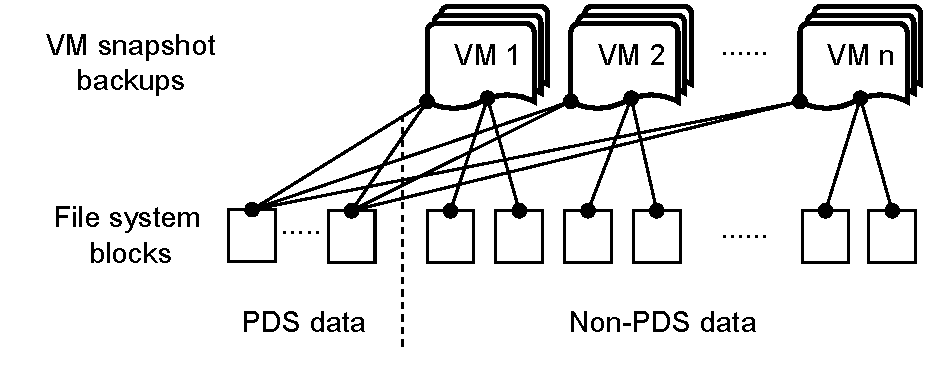
\includegraphics[width=4in]{images/share_vc}
        \label{fig:share_vc}
    }
    \\
    \subfigure[Sharing of file system blocks under VO]
    {
        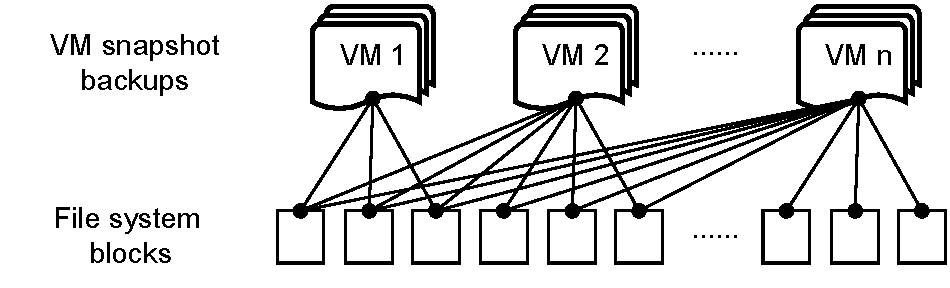
\includegraphics[width=4in]{images/share_vo}
        \label{fig:share_vo}
    }
    \caption{Bipartite association of VMs and file system blocks under (a) VC and (b) VO. }
    \label{fig:share}
\end{figure}

The replication degree of the backup storage 
is $r$ for regular file system blocks and $r=3$ is a typical setting in distributed
file systems~\cite{googlefs03,hdfs10}.
Since $\sigma$ is small (e.g.  2\% in our experiments),  
the impact of replication on storage increase is very small even 
when choosing  $r_c/r$ ratio as 2 or 3. 


%In the VC approach, a special replication degree $r_c$ is used for PDS data where $r_c>r$. 
%The storage cost for VO with full deduplication is $c_u *r$ and for VC, it is
%$ k*r_c  + (c-E(c-c_u))*r$. Thus The storage cost ratio of $VC$ over $VO$ is 
%\[
%\sigma \frac{r_c}{r} + \frac{c-e(c-c_u)}{c_u}.
%\]
%Since $\sigma$ is small (it is 2\% in our experiments),  
%term $\sigma \frac{r_c}{r}$ is small in the above expression.  
%Thus the impact on storage increase is very small even when we choose a large $r_c/r$ ratio. 
%For example, $r_c/r=2$ or 3. 

Now we  assess  the impact of losing $d$ machines 
to the VC and VO approaches.  
A large $r_c/r$ ratio can have a positive impact on full availability of VM snapshot blocks.
We use an FSB rather than a deduplication
data chunk as our unit of failure because the DFS keeps
file system blocks as its base unit of storage.
To compute the full availability of all snapshots of a VM, we derive
the probability of losing a snapshot FSB of a VM by
estimating the number of file system blocks per VM in each approach.
As illustrated in Figure~\ref{fig:share},
we build a bipartite graph representing the association from unique file system blocks
to their corresponding VMs in each approach. An association edge is  drawn  from an FSB to a VM 
if this block is used by the VM. 

For VC, each VM has an average number $N_1$ of non-PDS FSBs
and  has  an average of  $N_2$ PDS FSBs. 
Each non-PDS FSB is associated with one VM
 and  we denote that PDS FSBs are
shared by an average of $V_c$ VMs. 
%Let $s$ be the average number of chunks per file system block, 
%$V$ be the average number of VMs hosted on each machine. 
Then, 
\[
V pN_1 s  \approx c-E_c(c-c_u) - c_u\sigma\; \mbox{ and } \; 
V pN_2 s  \approx c_u \sigma V_c.
\]

For VO, each VM has an average of $N_o$ FSBs
and let $V_o$ be the average number of VMs shared by each FSB.
\[
V pN_o s  = (c- E_o(c-c_u) ) V_o.
\]

Since each FSB (with default size $64MB$) contains many chunks (on average 4KB),
each FSB contains the hot low-level chunks shared by many VMs, and it also contains
rare chunks which are not shared.  Since $c>> c_u$, from the above equations:
\[
\frac{N_1}{N_o} \approx  \frac{1-E_o}{(1-E_c) V_o}.
\] 
When $E_c$ is close to $E_o$,
%as demonstrated in Section~\ref{sect:evaldedup},
$N_1$ is much smaller than $N_o$. 
%When there is a failure in FSBs with replication degree $r$
%and there is no failure for PDS data with more replicas,   a VM in
%the VC approach has a much lower chance to lose a snapshot than VO. 
%Figure~\ref{fig:fsb-links} shows the average number of VMs sharing each file block from
%our test dataset.
%For VC, we only show
%the sharing degree of  PDS-oriented file blocs  because non-PDS blocks always belong to
%one VM.
%Figure~\ref{fig:fsb-links} shows the average number of VMs sharing each file block from our test data.
Figure~\ref{fig:vm-links} shows the average number of file system blocks for each VM in VC and in VO
and  $N_1$ is indeed  much smaller than $N_o$ in our tested dataset.  
%In fact, $N_1 +N_2 < N_o$. 
%This is likely because the PDS FSBs tightly pack data used by many VMs, 
%which decreases the overall number of FSBs required to backup a VM.
%Note that  if  the backup for multiple VMs were conducted concurrently, there could be many more
%VMs sharing each file block on average in VO. 

%Therefore, even when there is a loss of a PDS block, the VC approach tolerates the fault better.

\begin{figure}[htbp]
  \centering
	\begin{tikzpicture}
		\begin{axis}[
		%title={VO VM links},
                width=0.7\linewidth,
                height=0.5\linewidth,
		xlabel={Number of VMs},
		ylabel={Avg. Num. FSBs used by VM},
                xmin=0,
                ymin=0,
                xmax=106,
		%extra y ticks={4.5,5.5,6.5} %to show extra ticks
		%legend pos=north east,
                legend style={
                    at={(1,0.825)},
                    anchor=north east
                },
                %legend columns=3
		]
                \addplot[blue,mark=none] table[x=VMs,y=N_O] {data/vm_links_all.txt};
                %\addplot[red,dotted,mark=none] table[x=VMs,y expr=\thisrow{N_1}+\thisrow{N_2}] {figures/vm_links_all.txt};
                \addplot[red,dashdotted] table[x=VMs,y=N_1] {data/vm_links_all.txt};
                \addplot[red,densely dashed,mark=none] table[x=VMs,y=N_2] {data/vm_links_all.txt};
                \legend{$N_o$,
                    %$N_1+N_2$,
                    $N_1$,
                    $N_2$};
		\end{axis}
	\end{tikzpicture}
  \caption{Measured average number of 64MB FSBs used by a single VM. For VC both the number of PDS and Non-PDS FSBs used are shown.}
  \label{fig:vm-links}
\end{figure}

The full snapshot availability of a VM is estimated as follows with parameters $N_1$ and
 $N_2$ for VC and $N_o$ for VO.
Given normal data replication degree $r$, PDS data replication degree $r_c$, 
the availability of a file system block is the probability that  
all of its replicas do not appear in any group of $d$ failed machines among the total of $p$ machines. 
Namely, we define it as
\[
A(r) = 1-\binom{d}{r}/ \binom{p}{r}. 
\]
Then the availability of one VM's snapshot data under VO approach is the probability that
 all its FSBs are unaffected during the system failure:
%\begin{equation}
%\label{eq:VO}
%(1-\frac{ \binom{d}{r}} { \binom{p}{r} })^{N_o}. 
\[
A(r)^{N_o}. 
\]
%\end{equation}

For VC, there are two cases for $d$ failed machines.
\begin{itemize}
\item
When $r \le d<r_c$,  there is no PDS data loss and  
the full snapshot availability of a VM in the VC approach is 
%\begin{equation}
%\label{eq:VC1}
%(1-\frac{\binom{d}{r}} { \binom{p}{r} })^{N_1}.
\[
A(r)^{N_1}.
\]
%\end{equation}
Since $N_1$ is typically much smaller than $N_o$, 
the VC approach has a higher availability of VM snapshots than VO in this case.
%In the evaluation discussed in Section~\ref{sect:evaldedup}, 
%We have considered a worst case scenario where
%every PDS FSB is shared by all VMs in the VC approach, which leads a large $N_2$ value. 
%Even with $N_2$ being much higher than $N_o$ (as discussed below),
%the availability of VC snapshots is much higher than VO.

\item
When $r_c \leq d$, both non-PDS and PDS file system blocks in VC can have a loss.
The full snapshot availability of  a VM in the VC approach is
%\begin{equation}
%\label{eq:VC2}
% (1-\frac{ \binom{d}{r}} { \binom{p}{r} })^{N_1} 
% *
% (1-\frac{ \binom{d}{r_c}} { \binom{p}{r_c} })^{N_2}.
\[
A(r)^{N_1} * A(r_c)^{N_2}.
\]
%\end{equation}
%comparing  Formula~\ref{eq:VO} and~\ref{eq:VC}. 
\end{itemize} 
%In the evaluation discussed in Section~\ref{sect:evaldedup},
We have considered a worst case scenario that
every PDS FSB is shared by all VMs in the VC approach, which leads to a large $N_2$ value. 
Even with that, the availability of VC snapshots is still much higher than VO and  
there are two reasons for this:  1) $N_1$ is much smaller than $N_o$ as discussed previously.
2)  $A(r) < A(r_c)$ because $r < r_c$.  
Table~\ref{tab:fsb-availability} lists the $A(r)$ values with
%that the availability of an individual file system block
different replication degrees, to demonstrate the gap between  $A(r)$ and  $A(r_c)$.

% $1-\frac{ \binom{d}{r}} { \binom{p}{r} } < 1-\frac{ \binom{d}{r_c}} { \binom{p}{r_c} }$

\comments{
\begin{figure}[htbp]
  \centering
    \begin{tikzpicture}
            \begin{axis}[
                width=\linewidth,
                height=0.6\linewidth,
            %title={FSB Availability},
            cycle list name=mline,
            xlabel={Number of Machines Failed},
            ylabel={Availability of Single FSB (\%)},
            %extra y ticks={99.9}, %to add extra ticks
            mark options=solid,
            legend pos=south west,
            %legend columns=2,
            %legend style={
            %    at={(0.5,-0.2)},
            %anchor=north}
            ]
            \addplot table[x=NodesFailed,y=Availability5] {data/fsb_availability.txt};
            \addplot table[x=NodesFailed,y=Availability4] {data/fsb_availability.txt};
            \addplot table[x=NodesFailed,y=Availability3] {data/fsb_availability.txt};
            \legend{$R=5$,$R=4$,$R=3$};
            \end{axis}
    \end{tikzpicture}
    \caption{Availability of a file system block in a 100 machine cluster with different replication 
and failure settings.THIS PLOT WILL BE REPLACED BY TABLE}
  \label{fig:fsb-availability}
\end{figure}
}

\begin{table}
  \centering
    \footnotesize
    \tabcolsep=0.11cm
    \comments{%table data is obsolete, now uses pgfplotstable
        \begin{tabular}{|l|l|l|l|}
        \hline
        \multirow{2}{*}{Failures ($d$)}   & \multicolumn{3}{c|}{$A(r_c)\times 100\%$} \\
                                    %\cline{2-4}
                                    & $r_c=3$ & $r_c=6$ & $r_c=9$ \\
        \hline
        3 & 99.9994 & 100 & 100\\
        5 & 99.9939 & 100 & 100\\
        10 & 99.9258 & 99.9999 & 99.9999 \\
        20 & 99.2950 & 99.9967 & 99.9999 \\
        \hline
    \end{tabular}
    }
    \pgfplotstabletypeset[
        columns={NodesFailed,Availability3,Availability6,Availability9},
        columns/NodesFailed/.style={
            column name={\multirow{2}{*}{Failures ($d$)}}
        },
        columns/Availability3/.style={
            column name={\multicolumn{3}{c|}{$A(r_c) \times 100\%$}\\&$r_c=3$},
            fixed, precision=9
        },
        columns/Availability6/.style={
            column name={$r_c=6$},
            fixed, precision=9},
        columns/Availability9/.style={
            column name={$r_c=9$},
            fixed, precision=9},
        every head row/.style={
            before row={\hline},
            after row={\hline},
        },
        every last row/.style={after row=\hline},
        column type/.add={}{|},
        every first column/.style={column type/.add={|}{}},
    ]{data/fsb_availability.txt}
    \caption{$A(r_c)$ as storage nodes fail in a 100 node cluster.}
    \label{tab:fsb-availability}
\end{table}


\section{Approximate Snapshot Deletion with Leak Repair}
\label{data:deletion}

In a busy VM cluster, snapshot deletions can occur frequently.
Deduplication complicates the deletion process because space saving relies on the sharing of data
and it requires the global references to deleted chunks to be identified before they can be safely removed.
The complexity of our distributed environment obviates reference counting as an option,
and while the mark-and-sweep techniques can be used and optimization can be considered~\cite{Fabiano2013},
it still takes significant resources to conduct reference counting every time there is a snapshot deletion.
%
%In the case of Alibaba, snapshot backup is conducted automatically and there are 
%about 10 snapshot stored for every VM customer.
% Snapshot deletion can occur frequently, for example when there is
% a new snapshot created every day,  there will usually be a snapshot expired every day to maintain
% balanced storage use. 
%In addition, cloud users expect the reduced storage usage to be reflected
%instantly, which makes it difficult to adopt some resource efficient techniques such like perfect hashing\cite{Fabiano2013}.
We seek a fast solution with low resource usage to delete snapshots and
our VM-centric design simplifies the deletion process. 
Since PDS is small and separated, we can focus on unreferenced non-PDS chunks within each VM. 
%The PDS data chunks are commonly shared among all VMs and we do not consider them
%during snapshot deletion.  The selection of PDS data chunks is updated periodically independent of snapshot deletion process.
Another resource-saving strategy we propose is
an {\em approximate} deletion strategy to trade deletion accuracy for
speed and resource usage. Our method sacrifices a small percent of storage leakage
to efficiently identify unused chunks.

\begin{figure}
  \centering
  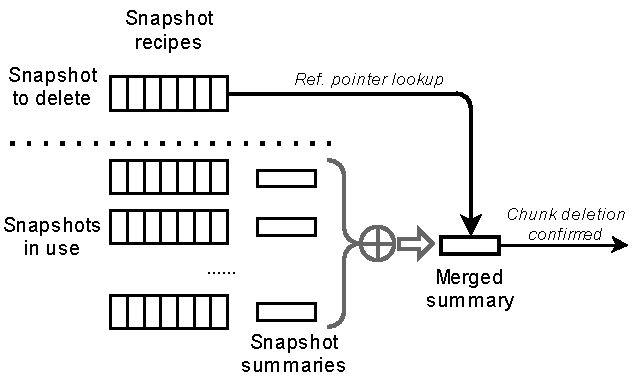
\includegraphics{images/deletion.pdf}
  \caption{Approximate deletion merges existing snapshot summaries to check block reference validity contained by a deleted snapshot}
  \label{fig:deletion_flow}
\end{figure}

We depict our approximate deletion process in Fig.\ref{fig:deletion_flow}, this procedure contains three aspects.
\begin{itemize}
\item {\bf Computation for snapshot reference summary.}
Every time there is a new snapshot created,
we compute a Bloom-filter with $z$ bits as the reference summary vector for all non-PDS chunks used 
in this snapshot.
The items we put into the summary vector are all the references appearing in the metadata of the snapshot.
For each VM we preset the vector size according to  estimation of VM image size,
given $h$ snapshots stored for a VM, there are $h$ summary vectors maintained.
We adjust the summary vector size and recompute the vectors if the VM size changes substantially over time.
This can be done during the periodic leakage repair stage described below.

\item {\bf Approximate deletion with fast summary comparison.}
When there is a snapshot deletion,  
we need to identify if chunks to be deleted from that snapshot
are still referenced by other snapshots. 
This is done approximately and quickly by comparing the 
reference of deleted chunks  with
the merged reference summary vectors of other live snapshots.
The merging of live snapshot Bloom-filter vectors uses the bitwise OR operator 
and the merged vector still takes $z$ bits.
Since the number of live snapshots $h$ is limited for
each VM, 
the time and memory cost of this comparison is small, linear to the number of chunks to be deleted.

If a chunk's reference is not found in the merged summary vector, we are sure that
this chunk is not used by any live snapshots, thus it can be deleted safely.
However, among all the chunks to be deleted, 
there are a small percentage of unused chunks  which
are misjudged as  being in use, resulting in storage leakage.

\item {\bf Periodic repair of leakage}.
%[exlpain why second Bloom filter, why scan append store]
Leakage repair is conducted periodically to fix the above approximation error.
This procedure compares the live chunks for each VM with what are truly used in the VM snapshot recipes.
A mark-and-sweep process  requires a scan of the entire snapshot store.
%Our VM-centric mark-and-sweep procedure is similar to Guo\cite{Guo2011} 
%in a way that the data dependency is clearly known.
%This generally requires a scan of almost the entire snapshot store which is much more expensive than approximate deletion,
%although certain optimized algorithms may apply\cite{Przemyslaw2013}. But 
Since it is a VM-specific procedure, 
the space and time cost is relatively small compared to the tranditional mark-and-sweep
which scans snapshot chunks from all VMs.
For example, consider each reference consumes 8 bytes plus  1 mark bit. A VM that has 40GB backup data with about
10 million chunks will need less than 85MB of memory to complete a VM-specific mark-and-sweep process
in less than half an hour, assuming 50MB/s disk bandwidth is allocated.
\end{itemize}

%{\bf Discussion}
We now estimate the size of storage leakage and how often leak repair needs to be conducted.
Assume that  a VM keeps $h$ snapshots in the backup storage, creates and deletes one snapshot
every day. Let $u$ be the total number of chunks brought by the initial backup for a VM, $\Delta u$ be the average
number of additional chunks added from one snapshot to the next snapshot version. Then the total number of 
chunks stored in a VM's snapshot store is about:
\[
U = u + (h-1)\Delta u.
\]

Each Bloom filter vector has  $z$ bits for each snapshot and let $j$ be the number of hash functions used by the
Bloom filter.  Notice that a chunk may appear multiple times in these summary vectors; however, this should not 
increase the probability of being a 0 bit in all $h$ summary vectors.
Thus the probability that a particular bit is 0  in all $h$ summary vectors is  
$(1- \frac{1}{z}) ^{j U}$. 
Then the misjudgment rate of being in use  is: 
\begin{equation}
\label{eq:falserate}
\epsilon = (1-(1-\frac{1}{z})^{jU})^j.
\end{equation}

For each snapshot deletion, the number of chunks to be deleted is nearly identical to the number of
newly added chunks $\Delta u$. 
Let $R$ be the total number of runs of approximate deletion between two consecutive 
repairs. We estimate  the total leakage $L$ after $R$ runs as:
\[
L = R \epsilon \Delta u.
\]

When leakage ratio $L/U$ exceeds a pre-defined threshold $\tau$, we trigger a leak repair. Namely,

\begin{equation}
\label{eq:leakrepair}
\frac{L}{U} = \frac{R \Delta u \epsilon}{u+(h-1)\Delta u } > \tau 
\Longrightarrow R > \frac{\tau}{\epsilon}\times\frac{u + (h-1)\Delta u}{\Delta u}.
\end{equation}

For example in our tested dataset,  
$h=10$ and each snapshot adds
about 0.1-5\% of new data. Thus we take ${\Delta u}/{u} \approx 0.025$. For a 40GB snapshot, $u\approx  10$ million.
Then $U=12.25$ million.
We choose  $\epsilon = 0.01$ and $\tau=0.05$.  From Equation~\ref{eq:falserate}, 
each summary vector requires $z=10U=122.5$ million bits or 15MB. From Equation~\ref{eq:leakrepair}, 
leak repair should be triggered once for every R=245 runs of approximate deletion. 
When one machine hosts 25 VMs and there is one snapshot deletion per day per VM, there would be 
only one full leak repair for one physical machine scheduled for every 9.8 days. 
If $\tau = 0.1$ then leakage repair would occur every 19.6 days.


\section{System Implementation and Experimental Evaluations}
\label{data:impl}
We have implemented and evaluated a prototype of our VC scheme on a Linux cluster of machines with
8-core 3.1Ghz AMD FX-8120 and 16 GB RAM. 
Our implementation is based on Alibaba cloud platform~\cite{Aliyun,WeiZhangIEEE}
and the underlying DFS uses  QFS with default replication degree 3 while the PDS replication degree is 6.
Our evaluation objective is to
study the benefit in fault tolerance and   deduplication efficiency of VC,  
and assess its backup throughput and  resource usage. 

We will compare VC with a VO approach  using stateless routing with binning (SRB) 
based on~\cite{Dong2011,extreme_binning09}.
SRB executes a distributed deduplication by routing a data chunk to one of cluster machines~\cite{Dong2011}
using  a min-hash function discussed in \cite{extreme_binning09}. Once a data chunk is routed to
a machine, the chunk is compared with the fingerprint index within this machine locally. 

\subsection{Settings}
We have performed a trace-driven study using a production dataset~\cite{WeiZhangIEEE} from 
Alibaba Aliyun's cloud platform with about 100 machines. 
Each machine hosts up to 25 VMs and each VM keeps 10 automatically-generated snapshots in the storage system while
a user may instruct extra snapshots to be saved.
The VMs of the sampled data set use popular operating systems such as 
Debian, Ubuntu, Redhat, CentOS, win2008 and win2003. 
%The backup of VM snapshots is required to complete within few  hours every night.
Based on our study of production  data,  each VM has about 40GB of storage  data  on average
including OS and user data disk.
%All data are divided into 2 MB fix-sized segments and 
The fingerprint for variable-sized chunks is computed using their SHA-1 hash~\cite{similar94,rabin81}. 
%Each segment is divided into 
%variable-sized content chunks with an average size of 4KB.
%Popularity of data blocks are collected through global counting and 
%and top popular ones ($\delta=2\%$)  are  kept in the PDS, as discussed in Section~\ref{sect:store}.

\subsection{Fault Isolation and Snapshot Availability}

 Table~\ref{tab:vm-availability} shows the availability of VM snapshots when 
there are up to 20 machine nodes failed in a 100-node cluster and  a 1000-node cluster. 
%Two VC curves use $V_c=1250$ and $V_c=2500$ representing the average number of VMs that share a PDS file system block. 
We have assumed a worst-case scenario that  a PDS block is shared by every VM. 
%($V_c=p*V$), which is to be expected when PDS
%blocks are sorted by hash, as their order is randomized.
%$V_c=2500$ represents  the absolute worst case for 2500 VMs. 
%The VO curve has  $V_o=6.3$ which is the average number of VMs that share a file system block in our smaller dataset.
%To get this number, we perform perfect deduplication over 105 VMs, append unique chunks to a DFS file and
%count the number of dependencies from a file system block to VM.
%In the scenario of having 2500 VMs, this number can only increase, thus this number represents the best
%case for VO approach. 
%Our results show that the VC approach even with $V_c=2500$ has a higher availability than VO.
%For example, with 10 machines failed, VO with 98.5\% availability would lose snapshots of 37 VMs 
%while VC with 99.9\% loses snapshots of 2.5 VMs.
%The key reason is that  $N_1 +N_2 < N_o$, caused by the fact that the VM-centric approach localizes deduplication
%and packs  data blocks for one VM as much as possible.  The extra replication
%for PDS blocks also significantly increases the snapshot availability even when
%a PDS file block is shared by every VM.
%=======
%Figure~\ref{tab:vm-availability} shows the availability of VM snapshots
%as storage nodes fail. 
%We assume a random distirbution of 64MB file system
%blocks (FSBs). where FSBs are not randomly distributed availability might
%be improved by limiting the number of storage nodes a particualr VM depends
%on but we take the conservative approach. We compare VO, the expected case for
%VC ($V_c=p*V/2$), and the worst case for VC ($V_c=p*V/2$). We set $V_o=6.3$
%based on measured values in our dataset.
%To obtain VO sharing of file blocks, we perform perfect deduplication over 105 VMs, 
%append unique chunks to a DFS file and
%count the number of dependencies from a file system block to VM.
%In the case of having 2500 or even 25000 VMs, this number can only increase, thus this number represents the best
%case for VO approach. 
Our results show that even the worst case,  VC  still has a significantly  higher availability than VO as the number of
failed machines increases.
%Our VM-centric approach shows significant improvements
%in VM availability.
For example, with 5/100 machines failed and 25 VMs per machine, VO with 93.256\% availability would lose data in 169 VMs 
while VC with 97.763\% loses data for 56 VMs.
The key reason is that for most data in VC, only a single
VM can be affected by the loss of a single FSB. Since most FSBs contain chunks for a single VM, VMs can depend on a smaller number of FSBs.
% because our VM-centric approach
%localizes deduplication.  

Although the loss of a PDS block affects many VMs,
by increasing replication for those blocks we minimize the effect on VM snapshot availability.
%By having extra replicas for the PDS data, we reduce the failure rate of PDS
%FSBs enough that the failure rate for the VM approaches the failure rate of the
%Non-PDS blocks. This minimizes the drop in availability between the expected
%and worst case for VC.
%
%One of the advantages of VC is that there is a division between
%popular and non-popular data to facilitate improved reliability. 
Figure~\ref{fig:pds-replication} shows
the impact of increasing PDS data replication. 
While the impact on storage cost is small, 
a replication degree of 6  has a significant improvement over 4, but the availability is about
the same for $r_c=6$ and $r_c=9$ (beyond $r_c=6$ improvements are minimal).

\begin{table}
  \centering
    \footnotesize
    \tabcolsep=0.11cm
    \pgfplotstabletypeset[
        columns={NodesFailed,VO100,VC100,VO1000,VC1000},
        columns/NodesFailed/.style={
            column name={\multirow{3}{*}{Failures ($d$)}}
        },
        columns/VO100/.style={
            column name={
                \multicolumn{4}{c|}{VM Snapshot Availability(\%)}\\&
                \multicolumn{2}{c|}{$p=100$}&\multicolumn{2}{c|}{$p=1000$}\\&
            VO},
            fixed, precision=6
        },
        columns/VC100/.style={
            column name={VC},
            fixed, precision=6},
        columns/VO1000/.style={
            column name={VO},
            fixed, precision=6},
        columns/VC1000/.style={
            column name={VC},
            fixed, precision=6},
        every head row/.style={
            before row={\hline},
            after row={\hline},
        },
        every last row/.style={after row=\hline},
        column type/.add={}{|},
        every first column/.style={column type/.add={|}{}},
        %the below rows can be used to extract rows 3,5,10,20 from rows 0-40
        %skip rows between index={0}{3},
        %skip rows between index={4}{5},
        %skip rows between index={6}{10},
        %skip rows between index={11}{20},
        %skip rows between index={21}{41}
    ]{data/availability_table.txt}
    \caption{Availability of VM snapshots for VO and VC.}
    \label{tab:vm-availability}
\end{table}


\begin{figure}[htbp]
  \centering
	\begin{tikzpicture}
		\begin{axis}[
                        width=\linewidth,
                        height=0.6\linewidth,
		%title={PDS Replication affect on availability},
		xlabel={Failed storage nodes},
		ylabel={VM Snapshot Availability (\%)},
                xmin=0,
                xmax=20,
		%extra y ticks={99.9}, %if important numbers are missing
                mark options=solid,
                legend style={
                    cells={anchor=west}, %legend entry alignment
                    legend pos=south west %legend position
                },
                reverse legend,
		]
                \addplot+[dashed] table[x=NodesFailed,y=VO]{data/node_failures_100.txt};
                \addplot table[x=NodesFailed,y=VC1]{data/node_failures_100.txt};
                \addplot table[x=NodesFailed,y=VC2]{data/node_failures_100.txt};
                \addplot table[x=NodesFailed,y=VC3]{data/node_failures_100.txt};
                \addplot table[x=NodesFailed,y=VC4]{data/node_failures_100.txt};
                \legend{
                    VO,
                    $r_c=4$,
                    $r_c=5$,
                    $r_c=6$,
                    $r_c=9$
                }
		\end{axis}
	\end{tikzpicture}
  \caption{Availability of VM snapshots in VC with different PDS replication degrees}
  \label{fig:pds-replication}
\end{figure}

\subsection{Deduplication Efficiency}
\label{sect:evaldedup}

%this version combines the old and the minhash alg. to compare against srb
\begin{figure}[ht]
  \centering
    \begin{tikzpicture}
            \begin{axis}[
            %title={Ex-Binning Efficiency},
            width=\linewidth,
            height=0.75\linewidth,
            cycle list={%
                {blue,solid,mark=square*},
                {blue,solid,mark=triangle*,mark size=1.5},
                {blue,solid,mark=diamond*,mark size=1.5},
                %{blue,solid,mark=pentagon*,mark size=1.4},
                {red,draw=red,dotted,mark=square},
                %{red,densely dotted,mark=triangle,mark size=1.5},
                %{red,densely dotted,mark=diamond,mark size=1.5},
                {brown,dashed,mark=*},
                %{red,densely dotted,mark=o},
                %{red,densely dotted,mark=pentagon,mark size=1.4},
            },
            mark repeat={10},
            xlabel={Number of VMs added},
            ylabel={Dedup. Efficiency (\%)},
            xmin=0,
            ymin=85,
            ymax=100,
            %extra y ticks={4.5,5.5,6.5} %to add extra ticks
            mark options=solid,
            legend pos=south west,
            legend columns=2,
            legend style={
                font={\tiny\sffamily},
                nodes={right}
                %at={(0.5,-0.2)},
                %anchor=north
            },
            ]
            \addplot table[x=VMs,y=MHcds4] {data/exbin_efficiency_comparison2.txt};
            \addplot table[x=VMs,y=MHcds2] {data/exbin_efficiency_comparison2.txt};
            %\addplot table[x=VMs,y=MHcds1] {data/exbin_efficiency_comparison2.txt};
            \addplot table[x=VMs,y=MHNocds] {data/exbin_efficiency_comparison2.txt};
            %\addplot table[x=VMs,y=cds4] {data/exbin_efficiency_comparison2.txt};
            \addplot table[x=VMs,y=cds2] {data/exbin_efficiency_comparison2.txt};
            %\addplot table[x=VMs,y=cds1] {data/exbin_efficiency_comparison2.txt};
            \addplot table[x=VMs,y=exbin] {data/exbin_efficiency_comparison2.txt};
            \legend{VC( $\sigma=4\%$),
                VC($\sigma=2\%$),
                %VC MH($\sigma=1\%$),
                VC(No PDS),
                %VC($\sigma=4\%$),
                VC($\sigma=2\%$\, No similarity guidance),
                %VC($\sigma=1\%$),
                SRB
            };
            \end{axis}
    \end{tikzpicture}
    \caption{Deduplication efficiency of VC and SRB.}
  \label{fig:exbin-efficiency-graph2}
\end{figure}

Figure~\ref{fig:exbin-efficiency-graph2} shows the deduplication efficiency for SRB and VC,
% <<<<<<< HEAD
% Our deduplication efficiency is defined as the percent of duplicate chunks
% which are detected and deduplicated, so only global perfect deduplication can have 100\% efficiency.
% The figure also compares several PDS sizes chosen for VC. ``$\sigma=2\%$'' 
% is defined in Table~\ref{tab:symbol}. 
% =======
namely the percent of duplicate chunks
which are detected and removed.
% so only global perfect deduplication can have 100\% efficiency.
% We also compare several PDS sizes chosen for VC.
%(see Table~\ref{tab:symbol} for definition of ``$\sigma=2\%$'')
%we allocate the space of distributed shared memory  to accommodate 2\%
%of data chunks shared among VMs, as defined in 
With $\sigma=2\%$, memory usage for PDS index lookup per machine is about 100MB per machine
and  the deduplication efficiency can reach over 96.33\%.
When $\sigma=4\%$, the deduplication efficiency can reach 96.9\% while space consumption increases to 200MB per machine. 
%and  the deduplication efficiency can reach 96.489\%.
%When $\sigma=4\%$, the deduplication efficiency can reach 97.027\% while space consumption increases to 200MB per machine. 
The loss of efficiency in VC is caused by the restriction of the physical memory available
in the cluster for fast in-memory PDS index lookup. 
%In the extreme case if we put all the fingerprint into PDS 
%index ($\sigma=100\%$) then VC will have 100\% efficiency.
SRB can deliver up to 97.79\% deduplication efficiency, which is slightly better than VC.
Thus this represents a tradeoff that VC provides better fault tolerance and fast approximate deletion
with competitive deduplication efficiency.

% SRB can deliver up to 97.935\% deduplication efficiency which is slightly better than VC.
% Thus this represents a tradeoff: VC provides better fault tolerance and fast
% approximate deletion with competitive (but slightly lower) deduplication
% efficiency.
% >>>>>>> 4dcd68612b052c0f890ed30361a9ed03771b5df1
%its loss of efficiency is caused by the routing of data chunks which restricts the search scope
%of duplicate detection.
%SRB provides slightly better deduplication efficiency than our VC approach, which we accept
%because we are rewarded by architecture-wise benefits such as fault-tolerance and fast 
%Though not our primary goal, this result does show that VC can remove competitive amount of duplicates.

Figure~\ref{fig:exbin-efficiency-graph2} also shows the curve  of VC without local similarity search.
There is a big efficiency drop in this curve when the number of VMs is about 30.
The reason is that  
%Without this (i.e. when we only 
there are VMs in which
data  segments are moved to another location on disk, for example when a file is rewritten
rather than modified in place,  
a dirty-bit or offset based detection would not be able to detect such a movement and 
similarity search becomes especially important.  We have found that in
approximately 1/3 of the VMs in our dataset this movement happens frequently.
In general, adding local similarity-guided search increases deduplication efficiency from 93\% to over 96\%.
That is one significant improvement compared to the work in ~\cite{WeiZhangIEEE}
which uses the parent segment at the same offset to detect duplicates instead of similarity-guided search.
% In general, our experiments show that
% dirty-bit detection at the segment level can reduce the data size to about 24.14\% of original data, 
% which leads about a 75.86\% reduction.
% Similarity-guided local search can further reduce the data size
% to about 12.05\% of original size, namely it delivers an additional 12.09\% reduction.
% The PDS-based global duplicate detection with $\sigma=2\% $
% can reduce the size further to 8.6\% of original size, namely it 
% delivers an additional 3.45\% reduction.

In general, our experiments show that
dirty-bit detection at the segment level can reduce the data size to about 24.14\% of original data, 
which leads to about a 75.86\% reduction.
Similarity-guided local search can further reduce the data size
to about 12.05\% of original, namely it delivers a 50.08\% reduction to the dirty segments.
The popularity-guided global deduplication with $\sigma=2\% $
can reduce the data further to 8.6\% of its original size, so
it provides additional 28.63\% reduction to the remaining data.

%Figure~\ref{fig:exbin-efficiency-graph2} also shows the benefits of our minhash
%similar segment search in the parent snapshot. 

\subsection{Resource Usage and Processing Time}

\comments{
\begin{table}
    \begin{tabular}{|c|c|}
    \hline
    PDS replication degree & Disk usage per machine  \\ \hline
    3                      & 3065GB             \\ \hline
    4                      & 3072GB             \\ \hline
    5                      & 3079GB             \\ \hline
    6                      & 3086GB             \\ \hline
    7                      & 3093GB             \\ \hline
    \end{tabular}
\caption{Storage space cost per machine for DFS under different PDS replication degree}
\label{tab:replication_cost}
\end{table}
}

{\bf Storage cost of replication.} 
%Table ~\ref{tab:replication_cost} shows the total storage space required by 
%VC as the PDS replication degree changes while non-PDS replication degree is fixed as 3. 
When the replication degree of both PDS and non-PDS data is 3, 
the total storage  for all VM snapshots in each physical machine takes about 3.065TB on average before compression
and 0.75TB after compression.  Allocating  one extra  copy for PDS data only adds  7GB in total per machine.
Thus PDS replication degree 6 only increases the total space by 0.685\% while PDS replication degree 9 adds 1.37\% 
space overhead, which is still small.
%The increase in storage cost is minimal because the PDS makes up a 
%small percent of the total storage space, while increasing replication degree has a  more significant benefit for
%availability as shown in Figure~\ref{fig:pds-replication}.

\begin{table}
  \centering
    \begin{tabular}{|c|c|c|c|c|c|}
    \hline
    Tasks & CPU & Mem &Read &  Write  & Time  \\ 
    & & (MB)          &(MB/s) &  (MB/s) & (hrs) \\ \hline
%    1     & 19\% & 118.1 & 50MB/s 8.37 & 1.314\\ \hline
    1     & 19\% & 118 & 50 & 16.4 & 1.31\\ \hline
%    2     & 35\% & 131.8 & 9.0 & 1.226\\ \hline
    2     & 35\% & 132 &50  & 17.6 & 1.23\\ \hline
    %4     & 63\% & 154.1 & 9.3 & 1.179\\ \hline
    4     & 63\% & 154&50   & 18.3 & 1.18\\ \hline
    6     & 77\% & 171.9 & 50 &  18.8 & 1.162\\ \hline
%    8     & 82\% & 90.5 & 89.2 & \\ \hline
%    10                      & 85\% & 97.2   & 90.4 \\ \hline
%    12                      & 91\% & 95.6    & 91.5 \\ \hline
    \end{tabular}
\caption{Resource usage of concurrent backup tasks at each machine}
\label{tab:resource_usage}
\end{table}

{\bf Memory and disk bandwidth usage with multi-VM processing}. 
We have further studied the memory and disk bandwidth usage 
when running concurrent VM snapshot backup on each machine with $\sigma=2\%$. 
Table ~\ref{tab:resource_usage} gives the resource usage  when
running 1 or multiple  VM backup tasks at the same time on each physical machine. 
``CPU'' column is the percentage of a single core used. 
``Mem'' column includes 100MB memory usage for PDS index and other space cost for executing deduplication tasks such as 
receipt metadata and cache. 
``Read'' column is controlled as 50MB/s bandwidth usage with I/O throttling so that other cloud services are not impacted too much.
The peak raw storage read performance is about 300MB/s and we only use 16.7\% with this collocation consideration.
``Write'' column is the I/O write usage of QFS and notice that each QFS write triggers disk writes in multiple machines due to
data replication.     50MB/s dirty segment read speed triggers about 16.4MB/s disk write for non duplicates with one backup task.
% [ NOT REASONABLE: Notice that memory and CPU used by PDS index and QFS are not included since they belong to 
% the cloud infrastructure services and are shared among many applications.]
%We see our hybrid deduplication scheme only occupies a small amount of system resources. 
%The  local deduplication only needs to keep the parent snapshot recipe and a few similar segment recipes in 
%memory during duplicate detection.

Table ~\ref{tab:resource_usage} shows that  a single backup task per node can complete the backup of the entire
VM cluster in about 1.31 hours. Since there are about 25 VMs per machine, we could execute
more tasks in parallel at each machine. But adding more backup concurrency does not shorten the overall time
significantly because of the controlled  disk read time.
%,  we can still process raw data at near 175 MB/s. If we consider the extreme case in which each machine has 25 VMs
%at 40GB size, our snapshot system can finish backing up all the VMs (1TB total) in 1.58 hours.

{\bf Processing Time breakdown}.
Figure~\ref{fig:vc_srb_combined} shows
the  average  processing  time of  a VM segment under VC and SRB. 
VC uses $\sigma=2\%$ and $4\%$.
It has a breakdown of processing time.
``Snapshot read/write'' includes snapshot reading and writing from disk, and 
updating of the metadata.
`` Network transfer" includes the cost of transferring raw and meta data from one machine to another during 
snapshot read and write.
``Index access/comparison'' is the disk, network and CPU time during fingerprint comparison.
This includes PDS data lookup for VC and index lookup from disk in VO after Bloom filter lookup.
For VC, the change of $\sigma$ does not significantly affect the overall backup speed as
PDS lookup takes only a small amount of time. The network transfer time for VC and SRB is about the same, because the 
amount of raw data they transfer is comparable.
SRB spends slightly more time for snapshot read/write because during each snapshot  backup, SRB involves many small bins,
 while VC only involves few containers with a bigger size. Thus, there are more opportunities for I/O aggregation in VC to reduce seek time.
SRB has a higher cost for index access and fingerprint comparison because most of  chunk fingerprints are routed
to remote machines for comparison while   VC handles most of chunk fingerprints locally. 

%on the index holding machine to access its index (often on the disk, supported by a Bloom filter) 
%and perform comparison.
%VC is faster in this regard because it conducts in-memory local search first and then
%accesses  the PDS on distributed shared memory, so most chunks can be dealt with locally.  
%SRB spends  slighter more time in  reading data and updates because it also updates the on-disk
%local meta data index in addition to partition indices.
%As a result Overall,  VC is faster than SRB, though data reading dominates the processing time for both algorithms.
%Figure~\ref{fig:vc_srb_combined} also reports the average backup time for a VM in VC when
%varying the PDS size.  It lists the time distribution for data reading,
%similarity-guided local search, global PDS lookup, and non-duplicate data writing. 
%While data reading dominates the backup process, PDS lookup spends about a similar amount
%of time as local search.

\begin{figure}[htbp]
  \centering
  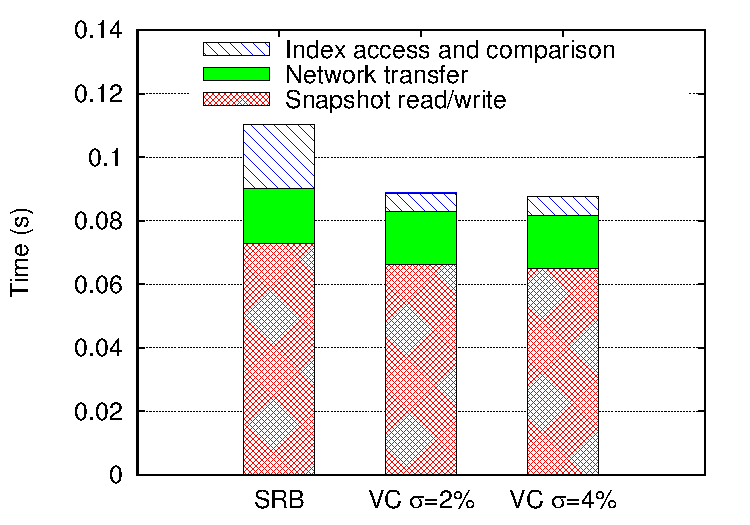
\includegraphics[width=4in]{figures/vc_srb_combined}
  \caption{Average time to backup a dirty VM segment under SRB and VC}
  \label{fig:vc_srb_combined}
\end{figure}

% \begin{figure}[htbp]
%   \centering
%   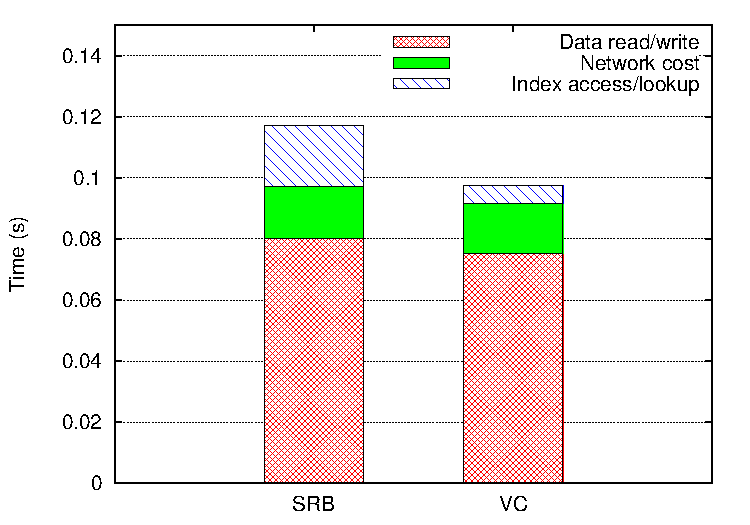
\epsfig{file=figures/srb_vs_vc, width=3in}
%   \caption{Time to backup a dirty VM segment under SRB and VC}
%   \label{fig:srb_vs_vc}
% \end{figure}


% \begin{figure}
%     \centering
%     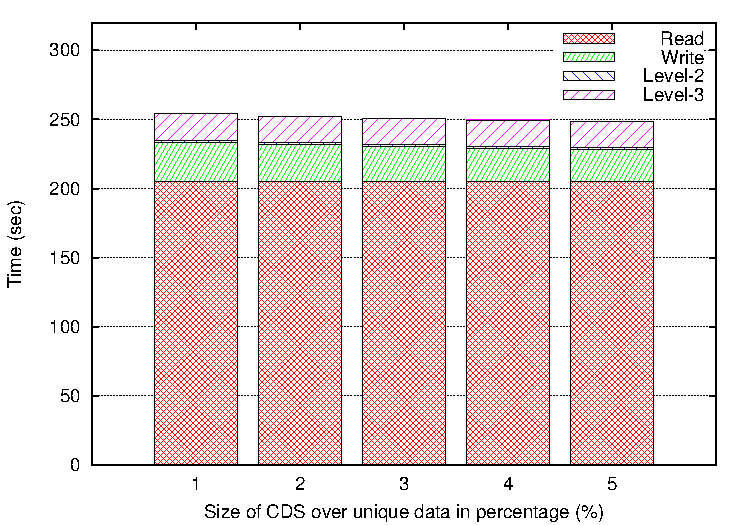
\includegraphics[width=3in]{figures/single_backup_time}
%     \caption{Average time to backup a VM in VC with varying PDS sizes}
%     \label{fig:single_vm_backup}
% \end{figure}


% \begin{table*}[t]
%     \centering
%     \begin{tabular}{c|ccc|ccc}
%     Num. of concurrent      & \multicolumn{3}{c|}{Throughput without}    & \multicolumn{3}{c}{Throughput with} \\
%     backup tasks            & \multicolumn{3}{c|}{I/O throttling (MB/s)} & \multicolumn{3}{c}{I/O throttling (MB/s)} \\ \cline{2-7}
%     per node                & Raw                                        & Snapshot Store & QFS  & Raw                                    & Snapshot Store & QFS  \\ \hline
%     1                       & 1369.6                                     & 148.0          & 18.0 & 171.3                                  & 18.5           & 2.26 \\
%     2                       & 2408.5                                     & 260.2          & 31.7 & 201.3                                  & 21.8           & 2.66 \\
%     4                       & 4101.8                                     & 443.3          & 54.1 & 217.8                                  & 23.5           & 2.87 \\
%     6                       & 5456.5                                     & 589.7          & 72.0 & 224.1                                  & 24.2           & 2.96 \\
%     \end{tabular}
% \caption{Throughput of software layers under different concurrency}
% \label{tab:throughput}
% \end{table*}
\begin{table}[htbp]
\centering
\begin{small}
    \begin{tabular}{|c|ccc|}
\hline
    Concurrent      & \multicolumn{3}{c|}{Throughput without}    \\
    backup tasks            & \multicolumn{3}{c|}{I/O throttling (MB/s)} \\ \cline{2-4}
    per machine                & Backup                                     & Snapshot Store & QFS  \\ 
    		&                                      & (write) & (write)  \\ \hline
    1                       & 1369.6                                     & 148.0          & 35.3 \\
    2                       & 2408.5                                     & 260.2          & 61.7 \\
    4                       & 4101.8                                     & 443.3          & 103.1 \\
    6                       & 5456.5                                     & 589.7          & 143.8 \\ \hline
    \end{tabular}
\end{small}
\caption{Throughput of software layers per machine under different concurrency}
\label{tab:throughput}
\end{table}

{\bf Throughput of software layers.}
Table~\ref{tab:throughput} shows the  average throughput of software layer
when when I/O throttling is not applied to control the usage.
%machine when all machine nodes execute one or multiple MV backup tasks.
``Backup'' column is the throughput  of the backup service  per machine.
``Snapshot store" is the  write throughput of the snapshot store layer. The gap between this
column and  ``Backup" column is caused by significant data reduction by dirty bit and duplicate
detection. Only non-duplicate chunks trigger a snapshot store write.
``QFS'' column is the write request traffic to the underlying file system after compression.
For example, with 148MB/second write traffic to the snapshot store, QFS write traffic is about 35.3MB/second
after compression.  The underlying disk storage traffic will be three times greater with replication.
The result shows that the backup service can deliver up to 5.46GB/second without I/O restriction
per machine with 6 concurrent backup tasks. With a higher disk storage bandwidth available, the above backup
 throughput would be higher. 
%With 50MB/second controlled I/O bandwidth, each machine can deliver 171MB/second with 1 backup task and can complete the backup of 25 VMs per machine in less than 1.31 hours.
 
%To begin, on each node we write snapshots for 4 VMs concurrently, and gradually 
%increase number of VMs to 12 to saturate our system capability. 
%We observed 
%the per-node throughput peaked at 2700 MB/s when writing 10 VM snapshots in parallel, 
%which is far beyond our QFS file system capability. The reason behind it is our efficient
%deduplication architecture and compression which greatly reduce the amount of data that needs to be written to
%the file system. The main bottleneck here is that our QFS installation only
%manages one disk per node, which prevents it from fully utilizing the
%benefits of parallel disk access. We expect our architecture can
%perform even better in production clusters, which often have ten or more disks on each node.


% \begin{figure}
%     \centering
%     \subfigure[Backup throughput per node under controlled I/O bandwidth usage]
%     {
%         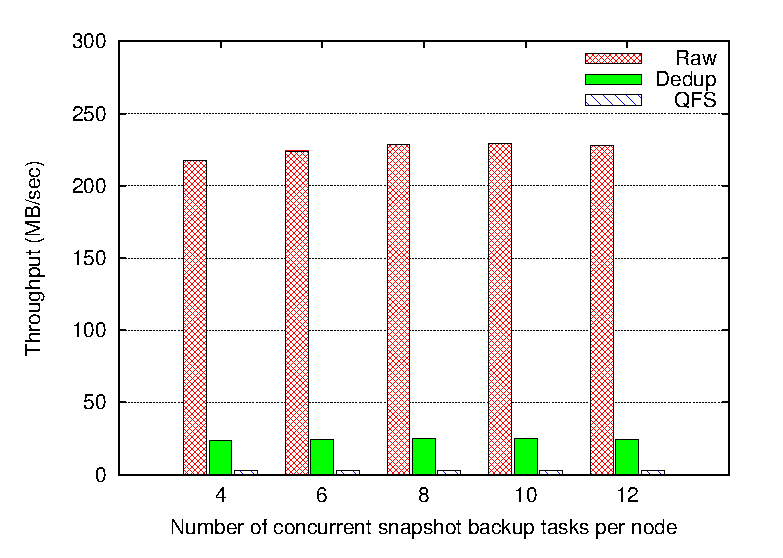
\includegraphics[width=3in]{figures/parallel_backup_with_read}
%         \label{fig:withread}
%     }
%     \\
%     \subfigure[Deduplication and storage system performance]
%     {
%         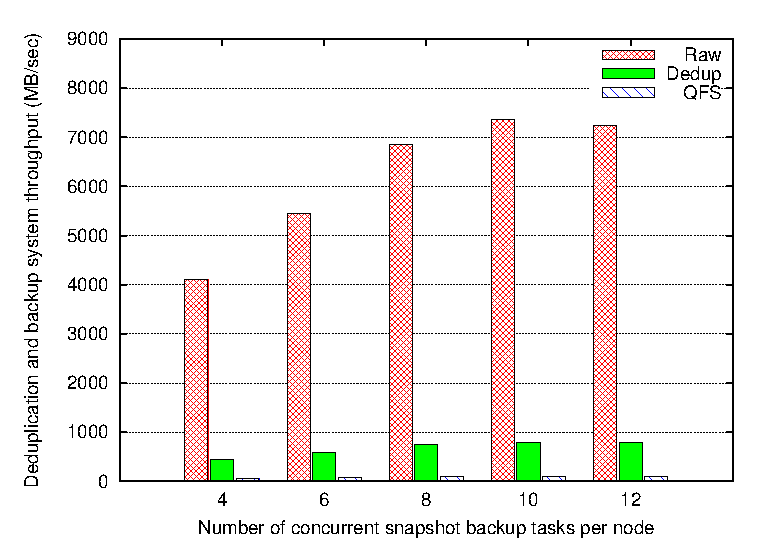
\includegraphics[width=3in]{figures/parallel_backup_no_read}
%         \label{fig:noread}
%     }
%     \caption{Throughput per-node with concurrent snapshot backup tasks}
%     \label{fig:parallel_backup}
% \end{figure}

 \subsection{Effectiveness of Approximate Deletion}

 \begin{figure}
     \centering
     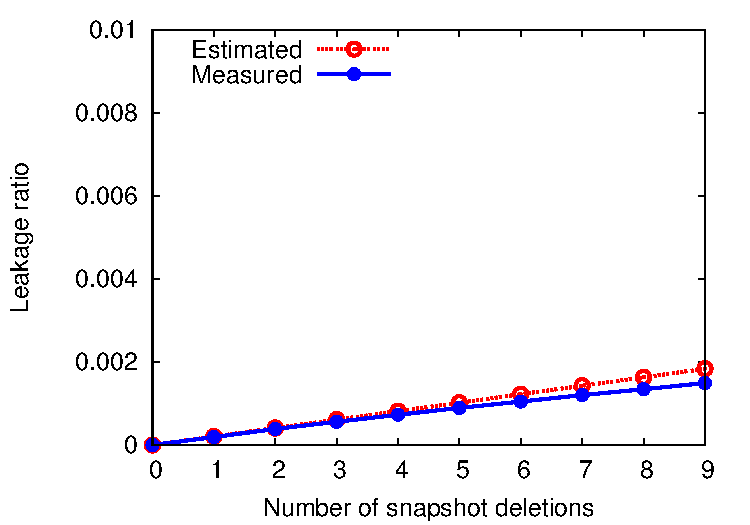
\includegraphics[width=4in]{figures/leakage}
     \caption{Accumulated storage leakage by approximate snapshot deletions ($\Delta u/u=0.025$)}
     \label{fig:leakage}
 \end{figure}

Figure~\ref{fig:leakage} shows the average accumulated storage leakage in terms of percentage of
storage space per VM caused  by approximate deletions.
The top dashed line is the predicted leakage using Formula~\ref{eq:leakrepair} from Section~\ref{data:deletion}
given $\Delta u/u=0.025$,
while the solid line represents the actual leakage measured during the experiment. 
The Bloom filter setting is based on $\Delta u/u=0.025$.
After 9 snapshot deletions, the actual leakage ratio reaches 0.0015 and this means that
there is only 1.5MB space leaked for every 1GB of stored data.
The actual leakage can reach  4.1\% after  245 deletions.


\section{Related Work}
\label{data:related}
Since it is expensive to compare a large number of chunk signatures for deduplication,
several techniques have been proposed to speedup searching of duplicate
fingerprints. For example, the data domain method ~\cite{bottleneck08} 
uses  an in-memory Bloom filter and a prefetching cache for data chunks  which may be
accessed.  An improvement to this work with parallelization is in ~\cite{MAD210,DEBAR,arrow08}.
The approximation techniques are studied in~\cite{extreme_binning09,Guo2011,WeiZhangIEEE}  
to reduce memory requirements with the tradeoff of a reduced deduplication ratio.
Additional inline deduplication techniques are studied in ~\cite{sparseindex09,Guo2011,Srinivasan2012}
and a parallel batch solution for cluster-based deduplication is 
studied in ~\cite{wei2013}. 
All of the above approaches have focused on optimization of deduplication
efficiency, and none of them have considered the impact
of deduplication on fault tolerance in the cluster-based environment that we have considered
in this work.

In designing a VC duplication solution, we have considered and adopted some of
the following previously-developed techniques.
1)
{\em Changed block Tracking}.
VM snapshots can be  backed up  incrementally by identifying data segments that have
changed from the previous version of the snapshot~\cite{Clements2009,Vrable2009,TanIPDPS2011,cvfs03}.
Such a scheme  is  VM-centric since deduplication is localized. 
We are seeking for a tradeoff since 
global signature comparison can deliver additional compression~\cite{Guo2011,Dong2011,extreme_binning09}.
2) {\em Stateless Data Routing}.
One approach for scalable duplicate comparison is to use a content-based hash
partitioning algorithm called stateless data routing by Dong et al.~\cite{Dong2011} 
Stateless data routing divides the deduplication work with a similarity approximation. This work 
is similar to Extreme Binning by Bhagwat et al.~\cite{extreme_binning09} and 
each request is routed  to a machine which holds
a Bloom filter  or can fetch on-disk index for additional comparison.
While this approach is VM-oblivious, it motivates us to  use  a combined signature of a dataset to narrow
VM-specific local search.
3) {\em Sampled Index}.
One effective approach that reduces memory usage is 
to use a sampled index with prefetching, proposed  by Guo and Efstathopoulos\cite{Guo2011}. 
The algorithm is VM oblivious and it is not easy  to adopt for a distributed architecture. 
To use a distributed memory version of the sampled index, every deduplication request
may access a remote machine for index lookup and the overall overhead of access latency for all requests
can be significant.  

\section{Concluding Remarks}
\label{data:concl}
In this chapter we propose a collocated backup service built on
the top of a cloud cluster to reduce network traffic and infrastructure requirements.
The key contribution is a VM-centric data management architecture that
integrate with multi-level deduplication to 
maximize fault isolation while delivering competitive deduplication efficiency.
Similarity guided local search reduces cross-VM data dependency and exposes more parallelism  
while global deduplication with a small common data set eliminates popular duplicates.
VM-specific file block packing also enhances fault tolerance by reducing data dependencies.
The design places a special consideration for low-resource usages as a collocated cloud service.
Evaluation using  VM backup data shows that VC strikes a tradeoff and 
can accomplish 96.33\% or 96.9\% of what complete global
deduplication can do.  The availability of snapshots increases substantially with 
a small replication overhead for popular inter-VM chunks.

We consider our approach has the potential to become a general purpose storage backend build
into the cloud to serve dropbox-like general file system backups. 